\documentclass[11pt]{article}
\usepackage{graphicx}
\usepackage{mathtools}
\begin{document}
\begin{titlepage}
\title{\Huge ECS 171 Final Report}
\author{\huge Aaun Abbas\\\huge Hilal Alsibai\\\huge Christopher Chen\\\huge Miguel Covarrubias\\\huge Jesse Dyer\\\huge Pei Guo\\\huge Alex Kot\\\huge Raymond Lau\\\huge Kent Wang\\\huge Ian Woods}
\maketitle
\end{titlepage}

\section{Abstract}
\paragraph{}
In this project, we compared the effectiveness of several machine learning classifiers at determining forest cover types from cartographic variables. The classifiers we used were artificial neural networks, k nearest neighbors, and random forests. Our results showed that random forests more accurately predicted the correct forest cover type than any other classifier. 
\section{Introduction}
\paragraph{}
Determining forest cover type from purely cartographic variables is important in situations where it is unfeasible or impossible to obtain cover type data through empirical methods. Thus, being able to accurately estimate the cover type of an area is of great interest to forest scientists \cite{blackard00}.  At the same time, the dataset provides a large amount of well structured data (581012 samples with 54 attributes) upon which different machine learning techniques can be tested and compared, making it an attractive dataset for computer scientists \cite{gama03,oza01,giannella,furnkranz,obradovic,klami}.
\par
Forest management and research relies on accurate cover inventory.  Traditionally, cover type data is recorded from the field.  This process is costly and is limited by property lines.  Predicting cover type from cartographic or remotely sensed data would allow forest managers and researchers to not only collect data from their land, but also to collect data from nearby private forests that may effect the target forest.
\par
Knowing forest cover allows researchers to predict risk of pathogen infection.  In California, researchers have used CALVEG data to estimate risk of Phytophthora ramorum infections, which target 23 specific host species \cite{ross04}.  Forest cover data can also be used to predict fire risk.
\par
UC Irvine's machine learning repository has a large forest cover dataset collected from Colorado's Roosevelt National Forest \cite{bache13}.  The dataset contains 54 features and a cover type from 581012 different 30 by 30 meter plots.  We chose to use this dataset because it contains information from cartographic variables only so our classifiers would not need potentially costly remote data inputs. Research on this particular dataset has compared Gaussian discriminant analysis with artificial neural networks (ANNs).  Discriminant analysis achieved $58\%$ classification accuracy and the ANN achieved $70\%$ classificaiton accuracy \cite{jock99}.  The ANN used by the researchers did not use feature selection or regularization and was trained without crossvalidation.  Training was done with a small subset of the data and each feature was considered which could have led to overfitting.

\section{Methods}
\paragraph{}
We use three different classifiers to determine forest cover type: artificial neural networks, k nearest neighbors, and random forests. The forest cover data set was found in UC Irvine's machine learning repository \cite{bache13}.  It contained 54 cartographical features from 581012 different 30 by 30 meter plots and assigned a forest cover type to each plot.  We merged the wilderness and soil type features, normalized the data, and then ran our classifiers.\\
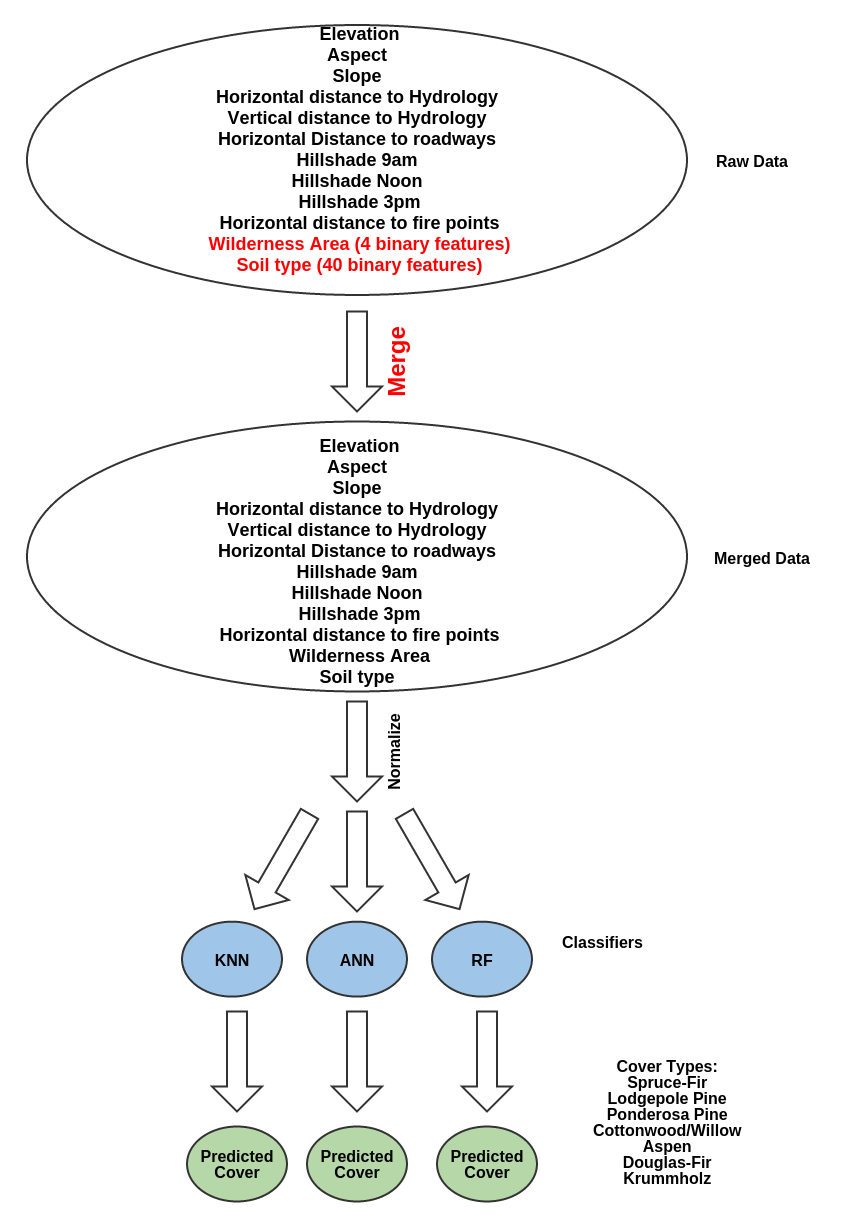
\includegraphics[width=\linewidth]{images/flow.png}

\subsection{Artificial Neural Networks}
\paragraph{}
We used a deep learning toolbox on Octave to implement a feed forward back propagation ANN with L2 regularization and multiple activation functions \cite{rbp12}.  ANNs with one hidden layer and two hidden layers were evaluated with 10-fold crossvalidation and the misclassification rate was used as the error. The settings were: learning $ \text{rate} = 1.5$, $\text{L2 penalty} = 0.0001$, $\text{number epochs} = 50$. We selected the ANN with the lowest misclassification rate as our classifier and used it to create both ROC curves and PR curves.  We created confusion matricies for each output node by iterating through threshold values.  From this we plotted the ROC and RP curves.  Finally, we took the predicted output for all our data through 10-fold crossvalidation and created a multiclass confusion matrix that details how classes were misclassified.
\subsection{k Nearest Neighbors}


\subsection{Random Forests}
\paragraph{}
We used Liaw and Wiener's R port \cite{liaw02} of Breiman's random forest algorithm \cite{breiman01}. Before training the classifier on the samples, we preprocessed the data so that the 4 boolean categorical variables that were related to wilderness area were rolled up into a single variable. We did the same for the 40 variables (also boolean categorical) that were related to soil type. This was done in order to speed up the training of the classifier.
\par
The random forest algorithm takes several parameters which control its speed and performance. We used empirical analysis to determine optimal values for these parameters. The first of these was $mtry$, which controls the number of variables that are sampled at each split when building the decision trees. 7 was determined to be the optimal value, as increasing the value past 7 caused almost no change in error, but consumed far more system resources. The other parameter was $ntree$ which controls the number of trees to be generated in the forest. For the same reasons as $mtry$, 40 was found to be the optimal value.
\par
To determine error, we used the OOB (out of bag) error \cite{breiman96}. We used this estimate because it is automatically generated by the algorithm while it runs, and because cross validation is not required when using OOB error, due to the way it is computed \cite{breiman01, breiman96}, which saved us computation time. It has also been shown to be close to an optimal estimate of the generalization error\cite{breiman96}.

\section{Results}
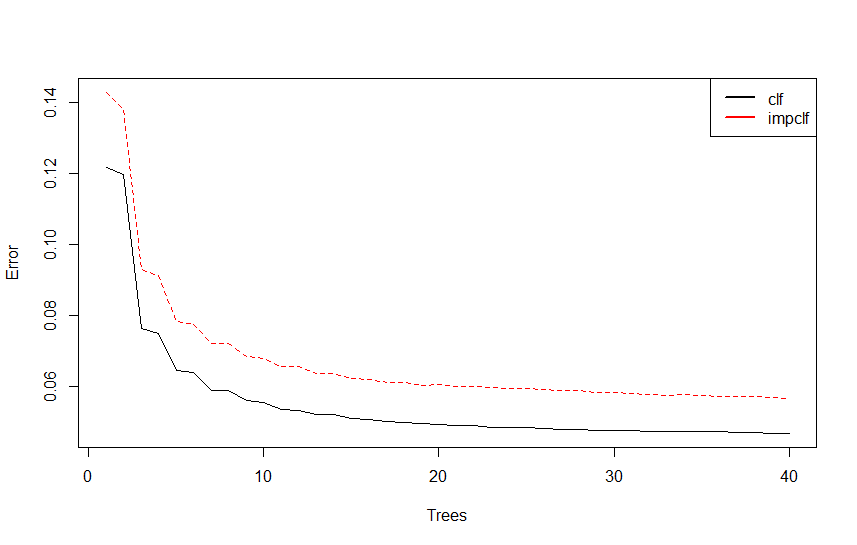
\includegraphics[width=\linewidth]{images/Rplot.png}
This should be an ROC curve.

We quickly found that the optimized tanh activation function outpreformed the sigmoid.  ANNs with one hidden layer had decreasing error until there were about 30 hidden nodes.  The one hidden layer structure did not do better $79\%$ accuracy. \\
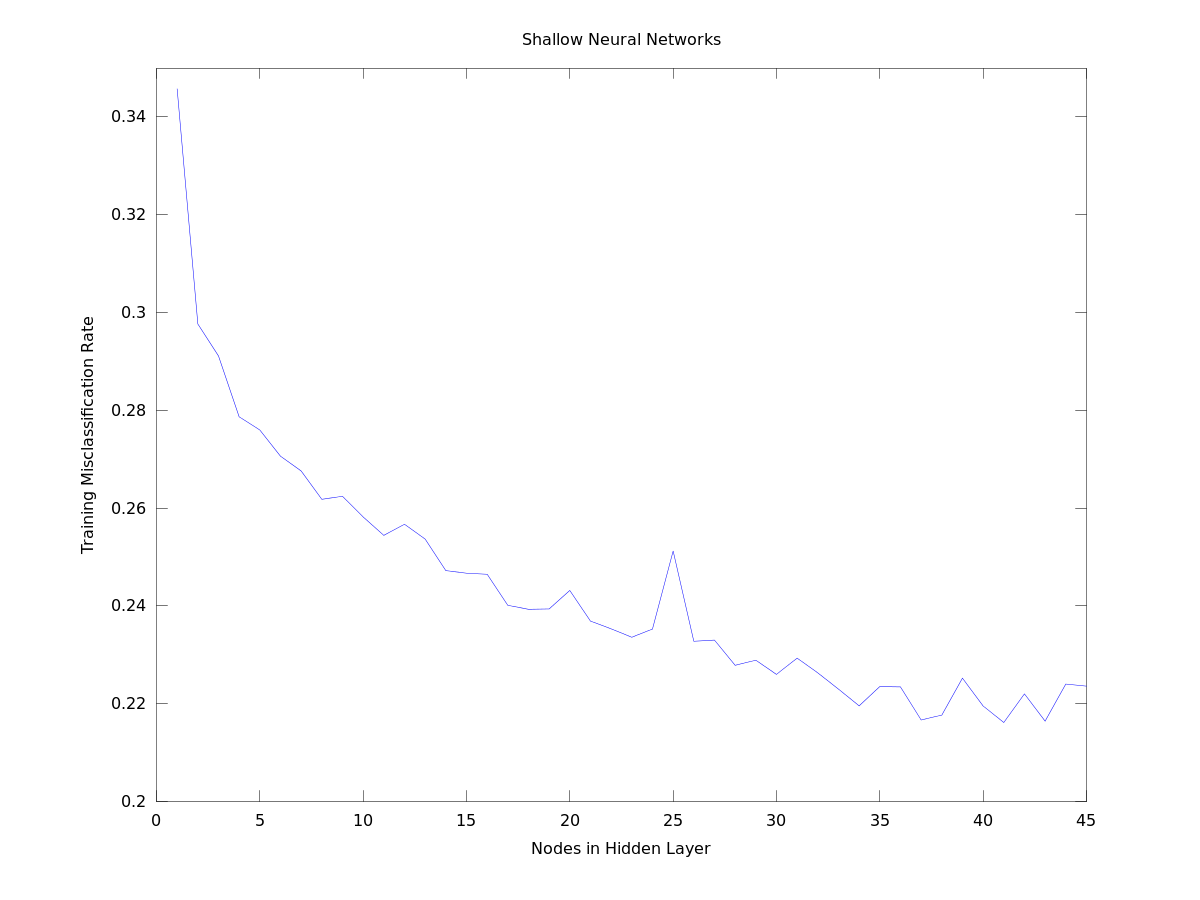
\includegraphics[width=\linewidth]{images/shallow.png}
ANNs with two hidden layers did slightly better with the best achieving $80.3\%$ accuracy.\\
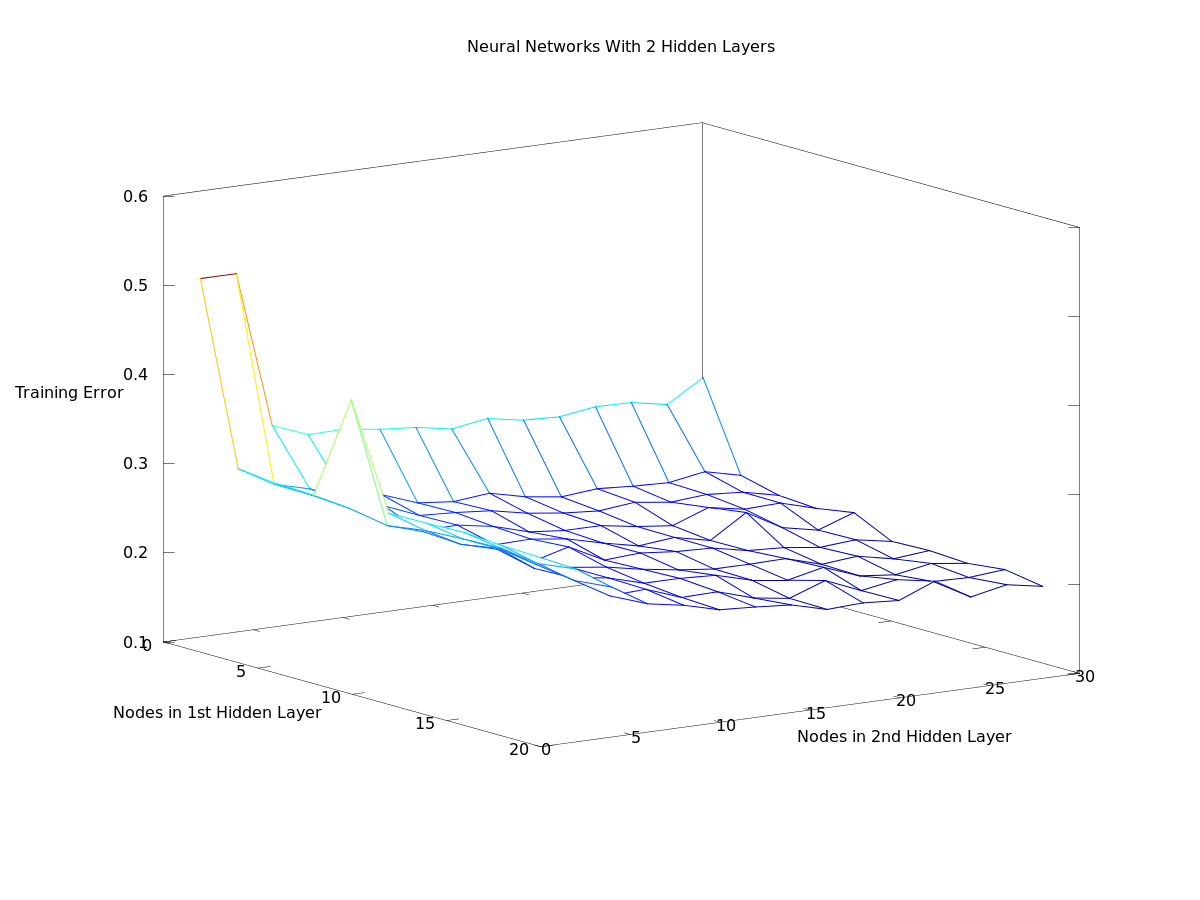
\includegraphics[width=\linewidth]{images/deep4.png}
This best structure had a first hidden layer with 19 nodes and a second hidden layer with 25 hidden nodes.  The ROC curves for this structure all have very high AUCs with the Aspen output node the lowest.\\
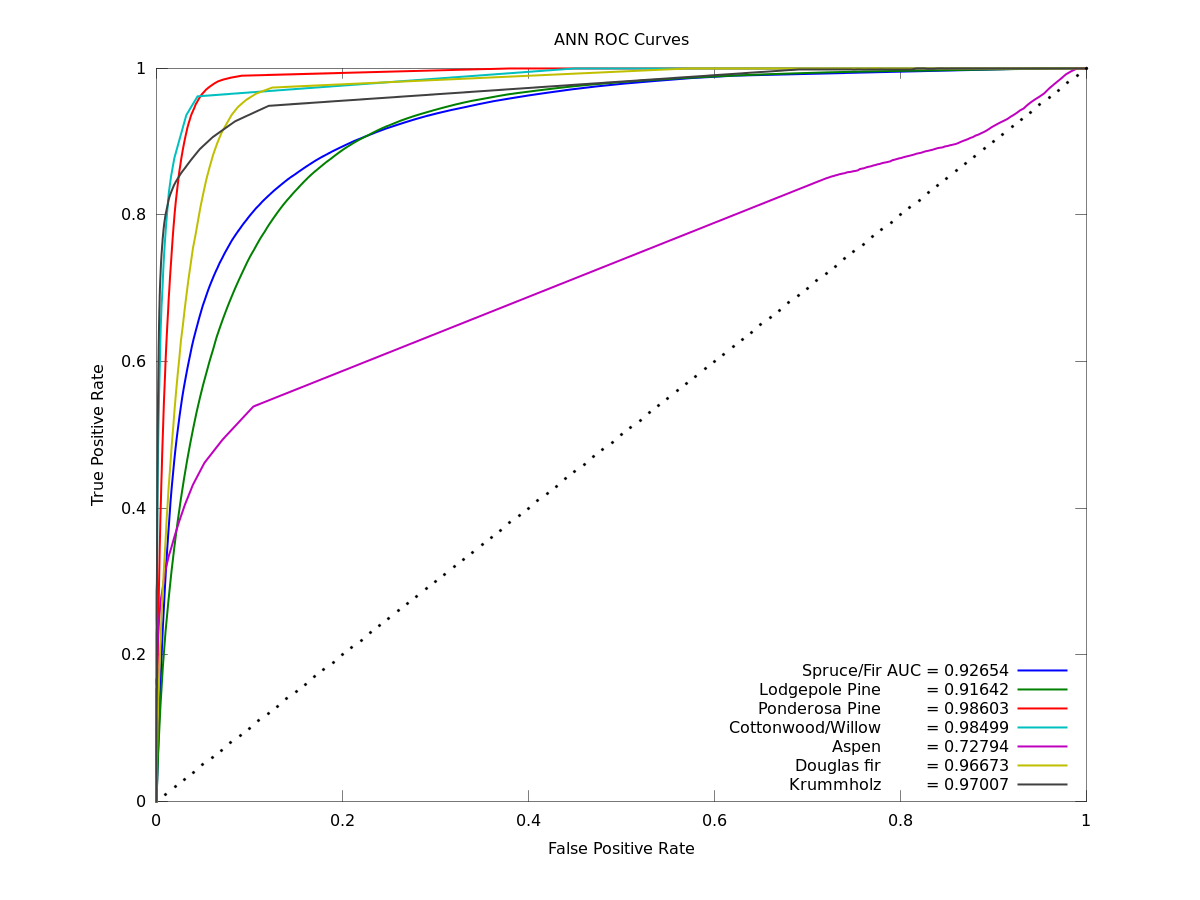
\includegraphics[width=\linewidth]{images/ROC_comp.png}
The PR curves are similar in that several output nodes have very high AUPRC values, with a few output nodes not doing as well. \\
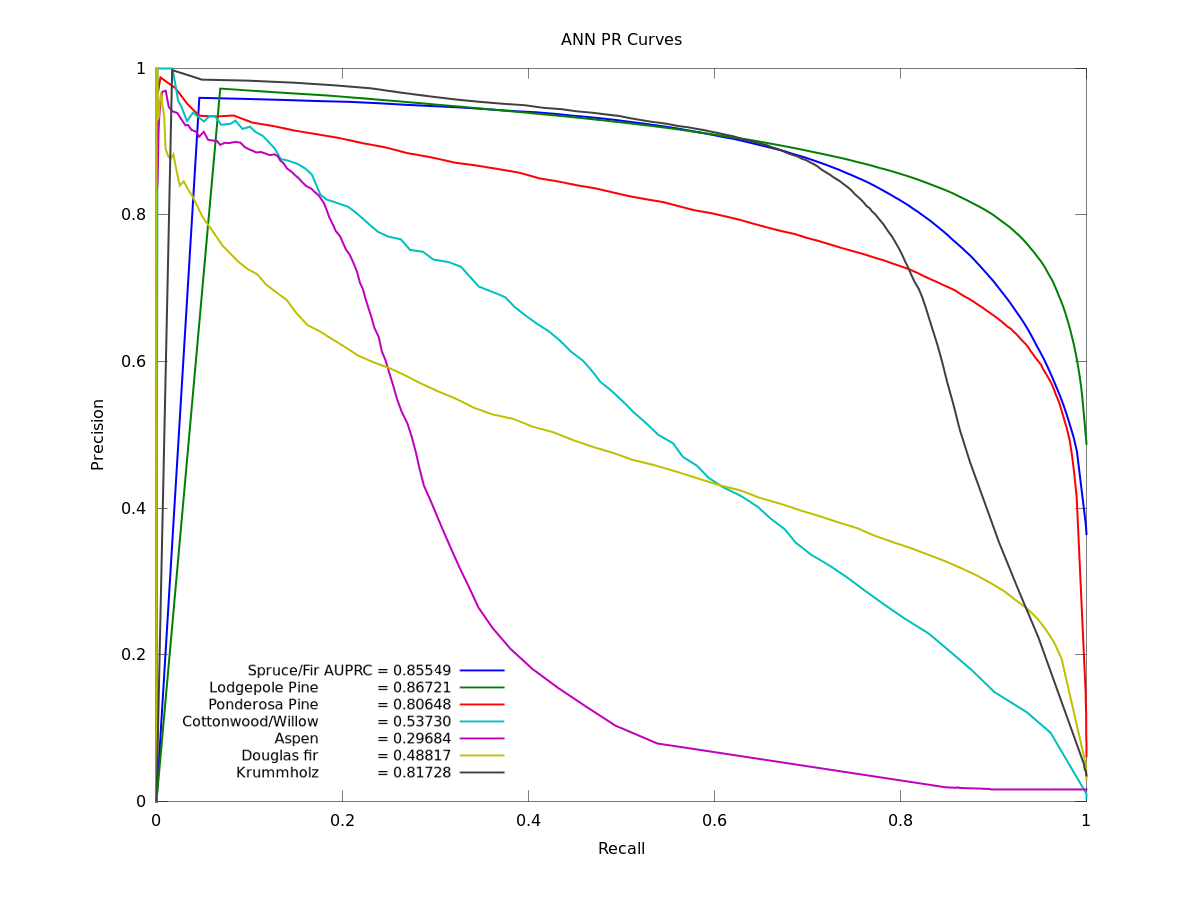
\includegraphics[width=\linewidth]{images/PR_comp.png} 
The multiclass confusion matrix revealed that there was a lot of misclassificaiton between Spruce and Lodgepole pine.  Cottonwood/Willow, Aspen, and Douglas-Fir were all misclassified the majority of the time.
\begin{center}
\begin{tabular}{|c | c| c| c| c| c |c| c|}
\hline
 & Observed& Observed& Observed& Observed& Observed& Observed& Observed \\ \hline
True Class & Sp.-Fir & L. Pine & P. Pine & C./Willow & Aspen & D.-Fir & Krum \\ \hline
Sp.-Fir & \textbf{166919} & 42605 & 16 & 3 & 47 & 34 & 2216 \\ \hline
L. Pine & 28706 & \textbf{250128} & 2821 & 8 & 310 & 996 & 330 \\ \hline
P. Pine & 22 & 3140 &  \textbf{30817} & 196 & 0 & 1579 & 0 \\ \hline
C./W. & 0 & 11 & 1671 &  \textbf{863} & 0 & 202 & 0 \\ \hline
Asp. & 471 & 7176 & 288 & 0 &  \textbf{1529} & 29 & 0 \\ \hline
D.-Fir & 124 & 4303 & 8558 & 110 & 1 &  \textbf{4271} & 0 \\ \hline
Krum. & 5031 & 518 & 0 & 0 & 0 & 0 &  \textbf{14961} \\ \hline
\end{tabular}
\end{center}

\section{Discussion}
\paragraph{}
Why is one classifier better than another?
The data has two classes that are over-represented with more than 200,000 observations and one class with less than 3,000 observations. \\
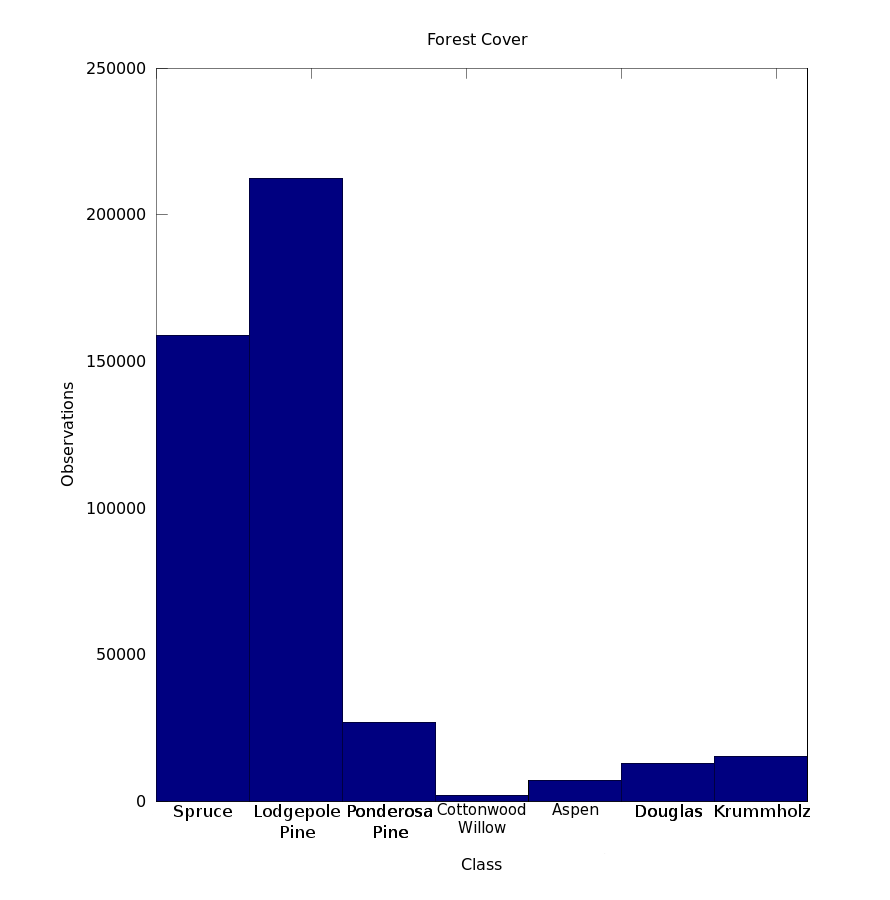
\includegraphics[width=\linewidth]{images/description.png} 
Pairwise analysis of the features revealed that no clear separation of classes existed.\\
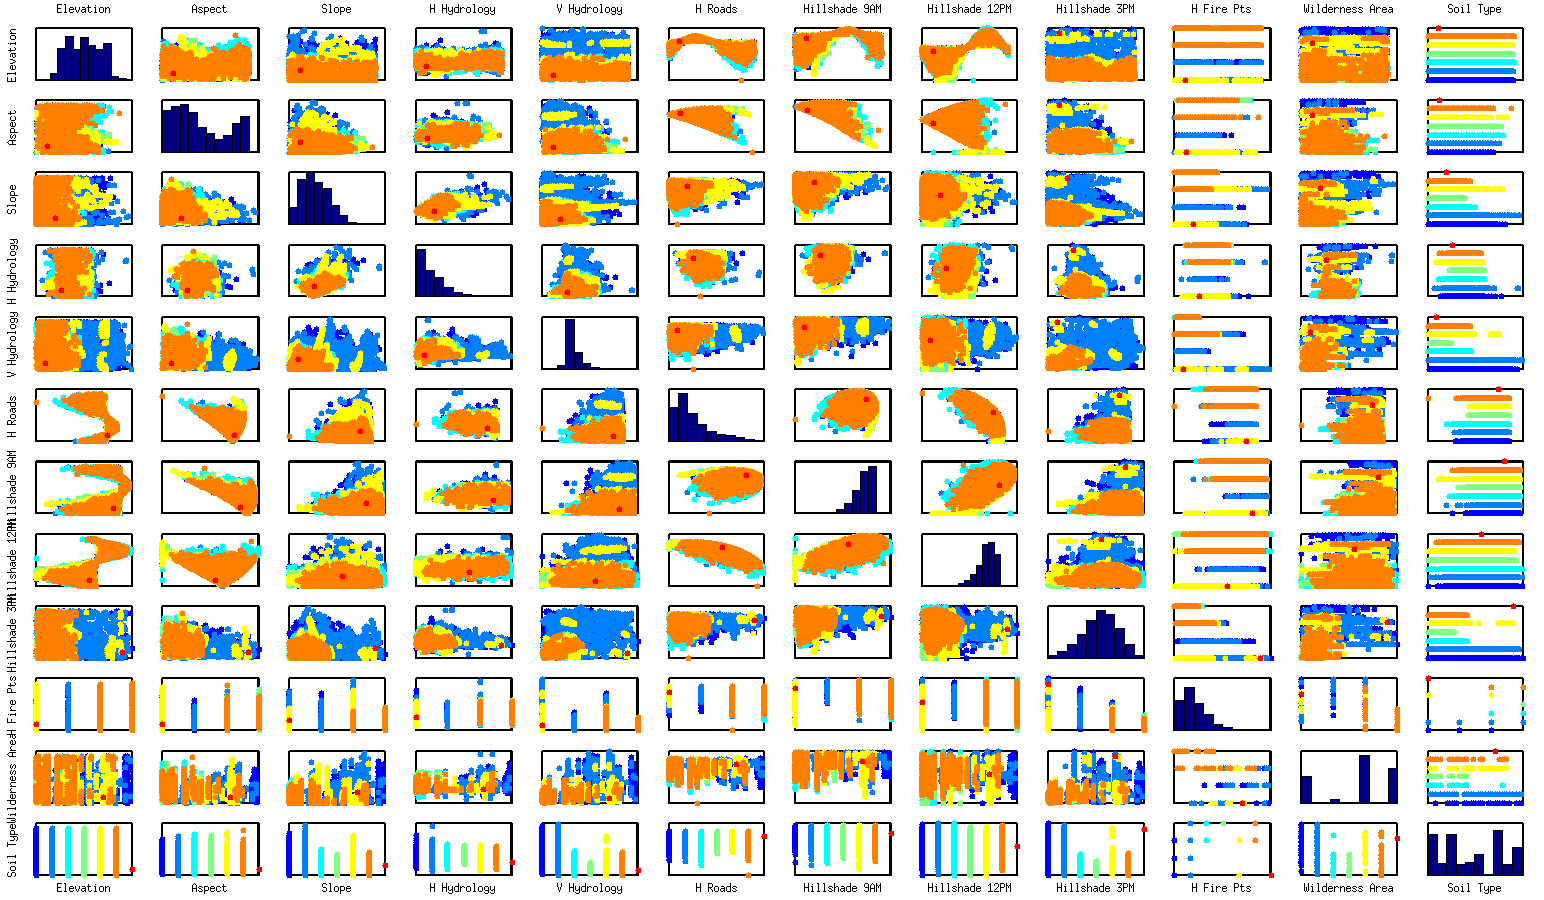
\includegraphics[width=\linewidth]{images/featureScatterPlotMatrixHD}
The optimized tanh activation function is a sigmoid that is centered around 0.\\
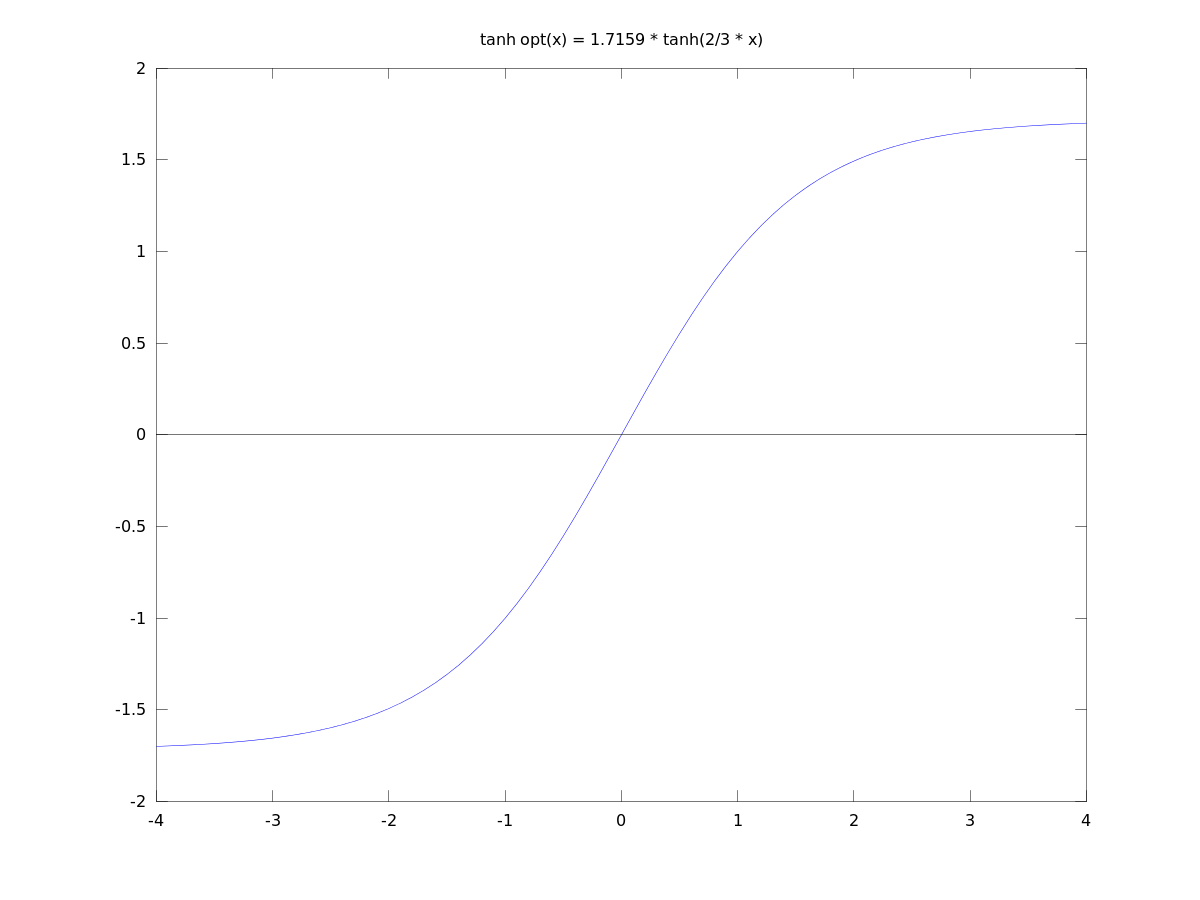
\includegraphics[width=\linewidth]{images/tanh}
This means that the average weights will be close to 0 and we will avoid overfitting.  Simillarly, L2 regularization will help to minimize the sum of weights by modifying the update rule to punish for large weights.  
\par
Our ANNs with single hidden layers did not learn the data very well.  Increasing the number of hidden layers slightly decreased the error.  We did do better than the existing ANNs to classify this dataset, which could be from using crossfold validation or the L2 regularization.  
\par
ROC analysis is not well understood in multiclass classification and extending the binary measure to a multicalss measure is computationally extensive \cite{lan07}.  Instead, we have split each of the output nodes into binary classifiers for separate analysis.  This allows us to analyze the classifier's preformance for each class type.
\par
Our ANN did not distinguish Cottonwood/Willow, Aspen, and Douglas-Fir very well.  This is likely from bias in the dataset as Spruce and Lodgepole pine are over-reprensented.  Most of our error came from the two over-represented classes, so we could train with different weights for each class to improve our classifier. 


\section{Conclusion}
In this project we used 3 different classifiers to predict forest cover type based on cartographic variables: artificial neural networks, k nearest neighbors, and random forests. We determined that random forests outperformed the other 2 classifiers. In the future, we may try to examine the performance of these classifiers on other datasets and then compare those results to those given here, or we may use different classifiers on the cover type dataset to see if we can improve our classification accuracy.

\section{Contributions}
Aaun Abbas and Raymond Lau wrote all of the code that was related to random forests. Christopher Chen wrote all parts of the report that were related to random forests.

\pagebreak
\begin{thebibliography}{}
\bibitem{blackard00}
Blackard, Jock A. and Denis J. Dean. 2000. "Comparative Accuracies of Artificial Neural Networks and Discriminant Analysis in Predicting Forest Cover Types from Cartographic Variables." Computers and Electronics in Agriculture 24(3):131-151.

\bibitem{gama03}
Joao Gama and Ricardo Rocha and Pedro Medas. Accurate decision trees for mining high-speed data streams. KDD. 2003.

\bibitem{oza01}
Nikunj C. Oza and Stuart J. Russell. Experimental comparisons of online and batch versions of bagging and boosting. KDD. 2001.

\bibitem{giannella}
Chris Giannella and Bassem Sayrafi. An Information Theoretic Histogram for Single Dimensional Selectivity Estimation. Department of Computer Science, Indiana University Bloomington.

\bibitem{furnkranz}
Johannes Furnkranz. Round Robin Rule Learning. Austrian Research Institute for Artificial Intelligence.

\bibitem{obradovic}
Zoran Obradovic and Slobodan Vucetic. Challenges in Scientific Data Mining: Heterogeneous, Biased, and Large Samples. Center for Information Science and Technology Temple University.

\bibitem{klami}
Arto Klami and Samuel Kaski and Ty n ohjaaja and Janne Sinkkonen. HELSINKI UNIVERSITY OF TECHNOLOGY Department of Engineering Physics and Mathematics Arto Klami Regularized Discriminative Clustering. Regularized Discriminative Clustering.

\bibitem{liaw02}
A. Liaw and M. Wiener (2002). Classification and Regression by randomForest. R News 2(3), 18--22.

\bibitem{breiman01}
Leo Breiman. Random forests. Machine learning 45 (1), 5-32. 2001.

\bibitem{breiman96}
Breiman, Leo. Out-of-bag estimation. Technical report, Statistics Department, University of California Berkeley, Berkeley CA 94708, 1996b. 33, 34, 1996.

\bibitem{bache13}
Bache, K. \& Lichman, M. (2013). UCI Machine Learning Repository [http://archive.ics.uci.edu/ml]. Irvine, CA: University of California, School of Information and Computer Science.

\bibitem{ross04}
Ross Meentemeyer, David Rizzo, Walter Mark, Elizabeth Lotz, Mapping the risk of establishment and spread of sudden oak death in California, Forest Ecology and Management, Volume 200, Issues 1–3, 25 October 2004, Pages 195-214, ISSN 0378-1127, http://dx.doi.org/10.1016/j.foreco.2004.06.021.
(http://www.sciencedirect.com/science/article/pii/S0378112704004463)

\bibitem{jock99}
Jock A. Blackard, Denis J. Dean. 1999. Comparative accuracies of artificial neural networks and discriminant analysis in predicting forest cover types from cartographic variables. Computers and Electronics in Agriculture. 24:131-51.

\bibitem{rbp12}
R. B. Palm. Prediction as a candidate for learning deep hierarchical models of data. 2012.

\bibitem{lan07}
Landgrebe TCW, Duin RPW. Approximating the multiclass ROC by pairwise analysis. 2007. Pattern Recognition LEtters 28:1747-58.



\end{thebibliography}
\end{document}